\subsubsection{Método do Chute}
O Método do chute consiste basicamente na substituição de um problema de valor de contorno por dois problemas de valor inicial. Para o caso de equações diferenciais ordinárias, com $ \Omega \subset \Re $ , o valor de  $ y(b) $ é obtido a partir da inclinação adequada da curva no ponto $ (a, \alpha) $. A figura ~\ref{fig:chute} ilustra este método.
\citep[p. 674]{burden_faires}


\begin{figure}[ht!]
\centering
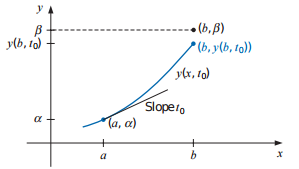
\includegraphics[scale=0.8]{figuras/Shooting.png}
\caption{Método do chute: o valor de $ \beta $ aproximado a partir da inclinação da derivada em $ (a, \alpha) $}
\label{fig:chute}
\end{figure}

